\documentclass{article}

\usepackage[french]{babel} 
\usepackage[utf8]{inputenc} 
\usepackage{color}
\usepackage{array} 
\usepackage[usenames, dvispnames]{xcolor} 
\usepackage{tikz}
\usepackage{tabularx}
\usepackage{graphicx}
\usepackage{lscape}

\title{Notes des différents papiers lus}
\author{Louisa Bessad}

\begin{document}

\maketitle
\tableofcontents
\newpage
\section{Chloé}
\subsection{SimGrid et SimterPose}
\textbf{SimGrid} est un simulateur d'applications distribuées en
environnement hétérogènes mais il implique de réécrire les
applications pour les modéliser.

\begin{itemize}
\item appl réelles nécessitent des plateforme, complexes et pas
  forcément reproductible (\textbf{Grid'5000})
\item simulation: modelisation d'applications et d'environnements,
  intéractions calculées via le simulateur, implique de reécrire
  l'application
\item {\color{red}emulation: applications réelles sur environnements
  virtuels}
\begin{itemize}
\item par dégradation \textbf{Distem}: ajoute une couche d'émulation
  au dessus de la plate-forme réelle mais diminue la capacité de
  l'hôte car il a joute un délai. Il n'est donc pas possible d'émuler
  des machines plus puissantes
\item par interception des actions (calcul, communications) de
  l'application \textbf{SimterPose}: exécution possible sur odinateur
  perso, ajout des délais de calcul via le simulateur et gestion du
  temps pour émuler des hotes plus puissants.
\end{itemize}
\end{itemize}

\textbf{Simterpose} permet d'utiliser \textbf{SimGrid} avec des
applications réelles, en faisant croire aux applications qu'elles
s'exécutent sur des machines distribuées. Il intercepte les actions
des applications réelles et les modifie:
\begin{itemize}
\item les calculs sont exécutés sur le PC réel et réinjectés les temps
  dans le simulateur
\item les communications sont modifiées pour imiter un environnement
  distribué, les délais (temps de calcul et connexion) sont calculés
  par le simulateur
\end{itemize}

L'interception des actions des applications se fait en utilisant deux
outils qui se complètent:
\begin{itemize}
\item ptrace: AS autorisant un processus à controler l'execution d 'un
  second (modification des registres d'un AS intercepté par exemple)
\item LD\_PRELOAD (éditeur de lien dynamique): interception au niveau
  de l'appel des bibliothèques. On va précharger des bibliothèques
  écrasant les fonctions à surcharger. {\color{red} risque de
    contournement si on oublie des fonctions}
\end{itemize}

Les AS ``time'', ``clock\_gettime'', ``gettimeofday'' avec
\textbf{ptrace} ne sont pas possibles, d'où l'alliance avec
LD\_PRELOAD.  SimterPose modifie les actions des applications et les
exécute en environnement virtuel, il simule des applications simples.

{\color{green} au lieu d'avoir des VM on a un simulateur proposé par
  SimterPose qui intercepte les actions de l'application}

SimterPose est une interface / API de SimGrid qui permet d'utiliser le
simulateur avec des applications réelles (sans avoir à les
réécrire). De plus on veut pouvoir tester les applications sans avoir
accès au code source. On teste les applications réelles sur une
plate-forme virtuelle simulée par SIMGRID. Les calculs sont réellement
exécutés sur la machine, les temps d'exécution injectés dans le
simulateur, les communications sont récupérées puis modifiées (permet
de remanier l'environnement vu par les applications). Les réponses à
ces deux points sont calculées par le simulateur.

ptrace est appelé à chaque entrée et sortie d'AS (considéré comme
point d'arrêt), cela permet aussi de pouvoir r/w directement en
mémoire des processus via \textbf{PEEK\_DATA POKE\_DATA}.

\subsection{Médiation}
Une action de l'application réelle appelle le simultaeur à calculer la
réaction de la plateforme virtuelle, on peut retarder le temps de la
phase de calcul ou de connexion et modifier la perception de
l'application en modifiant le temps. Simterpose doit lier les adresses
et les ports reseaux simulés avec ceux du réseau local, pour gérer
cela il existe deux solutions:
\begin{itemize}
\item Traduction d'adresse: le noyau gère les communications et
  modifie uniquement le tableau de correspondance d'adresse. On
  modifie les arguments que sont l'adresse et le port de
  connexion/communication.
\item Totale: l'application n'établit aucune connexion via socket avec
  une autre application, ptrace va directement écrire dans la mémoire
  du processus cible (on prend les arguments dans la mémoire de
  l'émetteur et on les écrit directement dans la mémoire du
  récepteur). On peut ainsi conserver les adresses simulées utilisées
  par les applications et on neutralise les AS de connexion.
\end{itemize}

\textit{LD\_PRELOAD permet de précharger des bibliothèques, on crée
  une bibliothèque dans laquelle on surcharge toutes les fonctions de
  temps et on exécute ces fonctions plutot que les originelles car
  ptrace ne permet pas de bien gérer les AS liés aux temps... Mais
  dans ce cas il ne faut pas oublier de fonction pour que le système
  ne passe pas au travers. SimterPose utilise l'API MSG.}

La traduction d'adresse surpasse la médiation totale, ce qui est
logique car les appels mémoires sont plus couteux. Les actions de
l'application sont interceptées et modifiées puis exécutées dans un
environnement virtuel simulé, c'est SimterPose qui fait cela et envoie
tout dans le simulateur SIMGRID (SURF).

\subsection{Reporting}
On écrit dans \textit{/proc/pid/mem} plutôt que \_PEEK. LD\_PRELOAD
s'applique directement sur write car tous les AS finissent par
l'appeler. Pour le temps on utilise la même technique que VDSO mais
avec LD\_PRELOAD (on lit une page partagée où SimGrid écrit l'heure
simulée et c'est ça qu'on renvoie à l'application notamment en le
mettant dans l'espace d'adressage du processus ``child''.

\section{Guillaume}
\subsection{AS}
Les AS sont constitués de 2 parties; la première consiste à
initialiser l'appel via l'application et à placer les valeurs des
arguments dans les registres du syscall. La seconde se fait après
l'exécution du syscall quand l'OS rend le controle à l'application
(les registres des arguments contiennent les anciennes valeurs reçues
en paramètre et on stocke la valeur du résultat dans le bon
registre). ptrace stoppe l'exécution du processus pour chacune de ces
parties afin de pouvoir récupérer toutes les informations qui
l'intéressent.

\subsection{Médiation}
With full mediation, applications don't use socket to comunicate,
there is no connexion either. The network address is the same that the
simulated address because there is no connexion.  In address
translation, every connexion and communication go through the kernel
to be routed but there is no traffic control from the OS. The
simulated address of the simultaed network is translated to
communicate in the local network. There is an array of the port used
by the application in the simulated world and in the reality and there
is bind between them. Because the same simulated port can be binded to
different real port.

SimterPose simulates a real network on a local network. In the address
translation, when we want to use some ports to have some connections,
we need to know if there are not used by another process. If not we
look for two real ports to bind them and store those links in an array
and we quit the syscall. When we want to receive or send something, we
check if there is something new to read before releasing the
read. With unblocking send we check if we receive something new to
send if not the application is not stopped, otherwise the send sends
the return value to the kernel which sends it to the simulator and
store it for reception mecanism and blocks the application which have
made the send. The address translation is limited by the number of
ports but extensions exist.

In full mediation the send is store in the memory so there is no
syscall blocked, we run the simultation and then release the
application. The receive check if there is something new or not to
block or not the application. The simulator stops the application when
the writing in the memory of the destination process is ended.
\begin{enumerate}
\item w in memory
\item is there something new?
\item if there is something we stops the application and we run the
  simulation until the end of the simulation, otherwise the
  application continues.  It allows to insure the consistency of the
  FD table of every process. The full mediation is bad with print
  memory.
\end{enumerate}

The address translation is more efficient for the exchange of big data
(because memory access to read something is heavy). But in real world
you don't have only it. In this way, full mediation is more efficent
for time problems (short data and many connections)

\subsection{Time}
The time for the application is the time of the simulator not the real
time. For the computation time we ask to the kernel and after this
time is given to the simulator.

\textit{On lance l'application sur l'hôte réel et on simule le
  déploiement sur la plateforme réelle} {\color{red} revoir page 22
  jusqu'à 27}

\section{Marion}
\subsection{3 techniques}
Pour déterminer le comportement exact d'une application sur un large
éventail de conditions environnementales on peut faire de l'exécution
sur plateforme réelle, de l'émulation ou de la simulation. La première
est une expérience \textit{in situ}, néanmomins cela oblige à avoir du
matériel disponible et n'est pas forcément reproductible du fait du
partage des ressources entre utilisateurs.

La simulation consiste à modéliser un système et à représenter une
application de façon théorique et mathématique pour l'exacuter dans le
système modélisé. Néanmoins même si elle est facile à mettre en \oe
uvre et facilement reproductible elle ne permet de valider qu'un
modèle de l'application et pas l'application réelle.

\begin{quotation}
L’émulation consiste à substituer un élément de l’environnement de
l’application par un logiciel. L’émulateur reproduit le comportement
d’un modèle dont toutes les variables sont connues.

Dans l’évaluation des applications distribuées, l’émulation est une
approche intermédiaire visant à résoudre les limitations de la
simulation : {\color{red} en émulant l’exécution de l’application sur
  une plate-forme virtuelle (simulée), il est possible d’exécuter
  l’application réelle sur une large gamme de conditions, dans un
  environnement entièrement contrôlé.} De plus, cela évite de devoir
développer 2 versions de l’application , l’une étant adaptée à
l’expérimentation sur simulateur tandis que la seconde est utilisée en
production. L’émulation d’applications réparties consiste à
intercepter les actions de l’application et à reporter ces actions
dans le simulateur.  Dans le cas d’une émulation offline , on
sauvegarde ces actions sur disque, puis on les rejoue après coup dans
le simulateur. Tandis que dans une émulation online , on reporte
immédiatement ces actions dans le simulateur, puis on retarde
l’application du temps calculé par le simulateur.

{\color{green} Le projet SimGrid[7] a débuté en 1999 pour permettre
  l’étude d’algorithmes d’ordonnancement sur des plateformes
  hétérogènes. Il s’agit d’un outil qui fournit des fonctionnalités de
  base pour la simulation d’applications distribuées hétérogènes en
  environnements distribués.  L’objectif spécifique du projet est de
  faciliter la recherche dans le domaine de la programmation
  d’applications distribuées et parallèles sur des plates-formes de
  calcul distribuée à partir d’un simple réseau allant du poste de
  travail aux grilles de calcul.

Le projet Simterpose s’insère dans un axe de recherche visant à
permettre l’étude sur simulateur d’applications complètes. L’objectif
est d’émuler en utilisant un simulateur, dans notre cas, SimGrid. On
souhaite ainsi fournir un émulateur simple et accessible à tous les
utilisateurs grâce à sa facilité de déploiement que ce soit sur un
simple ordinateur portable personnel ou bien sur un petit cluster. Un
tel émulateur doit permettre :
\begin{itemize}
\item l'exécution d’un grand nombre d’instances d’une application sur
  un même système en vue d’un debuggage ;
\item l’évaluation d’applications soumises à une large gamme de
  conditions telles que des caractéristiques d’un simple noeud ou d’un
  réseau complet différentes ;
\item la collecte d’information concernant le comportement de
  l’application pendant son éxecution
\end{itemize}
}
\end{quotation}

Les applications ne communiquent plus directement entre elles, lors
des communications c'est le simulateur qui va gérer les envois vers
les différentes stations en les analysant et effectuant parfois des
actions avant de transmettre les communications aux autres stations.

\begin{quotation}
Les objectifs sont d’étudier les moyens d’intercepter les actions des
applications et d’implémenter une méthode d’interception en
interagissant avec le simulateur SimGrid. Pour atteindre ce but,
plusieurs étapes sont définies. La première consiste à déterminer
combien de temps les actions d’une application mettent à se réaliser
sur la plateforme logique. La seconde consiste à intercepter les
actions de l’application ayant un impact sur son environnement.
\end{quotation}
On intercepte toutes les actions effectuées par chaque processus créés
par l'application. À chaque interception on génère une trace avec les
informations nécessaires pour le rejeu via le simulateur auquel on
envoie la trace. Les interceptions peuvent avoir lieu à plusieurs
niveaux:

\begin{quotation}
{\color{green} Un système d’exploitation est composé d’un ensemble de
  fonctions (les appels systèmes), elles-mêmes faisant appel aux
  fonctions internes du noyau. Dans les systèmes UNIX, on retrouve les
  appels POSIX où les prototypes des fonctions sont normalisés ainsi
  que les structures de données du système auxquelles elles
  accèdent. Enfin, juste avant le noyau, il y a les fonctions
  directement appelées par le noyau via les appels systèmes et
  inaccessibles au programmeur }
\end{quotation}

\begin{itemize}
\item application
\item bibliothèques (fonctions système de la libC et autres)
\item noyau
\end{itemize}

\subsection{Variable d'environnement: LD\_PRELOAD}
Éditeur de liens dynamiques de Linux permettant d'insérer du code dans
l'exécution d'un programme (interception au niveau de la couche
\textit{Bibliothèqes} du système).

\begin{quotation} 
{\color{green} La dernière phase de construction d’un programme est de
  réaliser l’édition de liens, ce qui consiste à assembler tous les
  morceaux du programme et de chercher ceux qui sont manquants.  Les
  fonctions utilisées par l’application sont fournies sous forme de
  bibliothèques. Lorsqu’on utilise une bibliothèque statique,
  l’éditeur de liens cherche le code dont l’application a besoin et en
  effectue une copie dans le programme physique généré. Pour les
  bibliothèques partagées, c’est le contraire : l’éditeur de liens
  laisse du code qui lors du lancement du programme chargera
  automatiquement la bibliothèque. Linux effectue par défaut une
  édition de liens dynamique s’il peut trouver les bibliothèques de ce
  type sinon, il effectue une édition de liens statique.  }
\end{quotation}

LD\_PRELOAD contient la liste des bibliothèques à précharger avant les
autres, ainsi en insérant notre bibliothèque dans cette variable
d'environnemenr ce seront nos fonctions qui seront utilisées et pas
les fonctions initiales du système. Néanmoins il ne faut pas oublier
de fonctions sinon l'application pourrait contourner notre
système. Pour intercepter l'appel de fonction d'une bibliothèque il
faut créer une nouvelle version portant le meme nom, comme dans notre
cas nous ne souhaitons pas empecher l'AS mais juste l'intercepter nous
ferons appel à la fonction originelle dans notre nouvelle fonction (en
utilisant les fonctions de la famille dlopen). Ensuite on compile le
fichier pour obtenir un .so contenant nos nouvelles fonctions et on
l'insère dans la vairable d'environnement avant l'exécution (notre
bibliothèque sera donc prioritaire \textit{cf exemple}).

\begin{quotation}
{\color{green} Cette approche permet donc de modifier le comportement
  d’une application de façon indirecte, sans avoir à recompiler ou
  rééditer les liens à chaque fois. De plus, les applications
  distribuées étant généralement multi-process, il faut garantir une
  interception pour les éventuels nouveaux processus créés, ce que
  fait directement LD\_PRELOAD sans ajouter d’option
  particulière. Cependant, cette approche s’avère vite incomplète dans
  notre cas puisqu’elle ne permet que de surcharger les fonctions des
  bibliothèques mais pas des appels systèmes. On n’obtient donc pas de
  réelle interception et nous n’avons aucune garantie que le système
  ne va pas contourner la nouvelle bibliothèque pour aller directement
  à la couche des appels systèmes}
\end{quotation}

\subsection{AS ptrace (lié au noyau)}
Cet AS permet d'accéder en r/w à tout l'espace d'adressage d'un
processus (données, strcutres de controle: registre du processeur par
exemple). Pour cela on crée un processus parent qui contrôle
l'exécution d'un autre processus et peut modifier son image
mémoire. Pour cela on fournit les requêtes que l'on souhaite voir
exécuter en paramètre de l'AS, les actions peuvent se faire sur les
deux processus (le traceur et le tracé). Pour utiliser cette appel et
suivre une application il faut:
\begin{enumerate}
\item créer le processus à tracer (fils) et le traceur (père) en
  utilisant fork()
\item le fils indique qu'il veut etre tracé grace à la requête
  \textbf{PTRACE\_TRACEME} puis ecécute l'application avec exec. Si le
  processus fils existe déjà le père s'y attache directement avec la
  requête \textbf{PTRACE\_ATTACH}.
\item Pendant l'exécution de l'application le père peut soit laisser
  le fils s'exécuter et prendre la main quand il reçoit un signal ou
  être interrompu pas à pas à chaque exécution d'instruciton ou d'un
  AS. Le processus fils s'arrêtera donc à chaque fois qu'il délivrera
  un signal et le père sera notifié lors de son prochain wait et
  pourra inspecter, modifier le fils arrêté puis reprendre l'exécution
  de son fils.
\item Quand le père a terminé de tracé le fils, il peut choisir de le
  terminer avec la requête \textbf{PTRACE\_KILL} ou le laisse
  continuer sans le suivre avec la requête \textbf{PTRACE\_DETACH}.
\end{enumerate}

\begin{quotation}
\textit{cf example} {\color{green} Du point de vue du niveau
  d’interception, ptrace() est donc lié au noyau. Ceci implique un
  éventuel problème de portabilité. En effet, il n’est pas assuré de
  pouvoir lancer une application écrite pour une version (majeure)
  différente du noyau : la mémoire virtuelle vue par un processus peut
  avoir été complètement remaniée, les alignements, la taille d’un mot
  peut changer ou bien encore, la sémantique de certains signaux peut
  avoir été modifiée, etc ... . De même, entre différentes
  architectures, il est difficile d’assurer une quelconque
  compatibilité : les registres changent, leurs tailles, la capacité
  du processeur à accéder à des adresses mémoires non alignées, etc
  ...  }
\end{quotation}
Néanmoins ptrace implique de bloquer l'application contrairement à
uprobes.

\begin{tabular}{|c|c|c|}
\hline & LD\_PRELOAD & ptrace\\ \hline Niveau d'interception &
Bibliothèques & Noyau \\ \hline Cout & Faible & Moyen \\ \hline
Facilité d'utilisation & Simple & Assez complexe \\ \hline
\end{tabular}

/usr/include/asm/unistd\_64.h

\subsubsection{ptrace et les registres}
ptrace utilise les registres de données pour stocker les arguments des
fonctions et leur résultat. Pour les manipuler il faut utiliser la
requête \textbf{PTRACE\_GETREGS} qui recupère l'ensemble des registres
et leur contenu dans une structure \textit{user\_regs\_strcut}. S'il
ne s'agit pas de fonctions liées aux sockets on peut lire les
arguments directement en lisant le contenu des registres. Dans le cas
des fonctions gérant les sockets on utilise un AS particulier à 2
arguments \textbf{socketcall}. Le premier est le numéro de la
sous-fonction de socket à exécuter et le deuxième est l'adresse du
segment mémoire contenant les arguments pour cette sous
fonction. Ainsi le second registre contient une adresse mémoire à lire
et on parcourt ensuite les adresses mémoires suivantes pour récupérer
tous les arguments, pour cela on a la requête
\textbf{PTRACE\_PEEKDATA}, qui lit un mot à une adresse mémoire donnée
dans l'espace d'adressage du processus fils, de ptrace.
\begin{quotation}
La difficulté avec cette opération est le déplacement dans la mémoire
où chaque case est de taille sizeof(long).
\end{quotation}

\subsubsection{ptrace et les temps d'exécution}
En plus des AS il faut fournir à SimGrid le temps d'exécution pour
qu'il les prenne en compte dans son analyse.
\begin{quotation}
La difficulté dans ce calcul était de différencier les différents CPU
time de chaque processus dans le cas de multithreading. Ainsi, pour
chaque processus tracé, on a une structure contenant les derniers CPU
time et Wall time calculés, les valeurs totales n’étant pas stockées
car elles sont recalculées à chaque interruption.
\end{quotation}

\subsection{Communications entre processus}
\subsubsection{Identification des entités communicantes}
Pour identifier les processus qui communiquent entre eux on ne peut
pas se contenter d'identifier le FD associé à la socket car chaque FD
est unique pour UN processus, mais il peut-être réutilisé par tous les
autres puisqu'ils ont chacun leur propre espace mémoire et donc leurs
FD. Ainsi il faut utiliser le FD, l'IP locale et distante et les ports
locaux et distants utilisés, on lie ensuite le FD de la socket à ces
informations pour savoir quels porcessus communiquent entre eux.

Pour effectuer des communications entre processus il faut d'abord
créer une socket. Ensuite dans le cas d'un serveur on utilisa la
fonction bind qui associe à une socket une @IP locale et un port (
``assignation d'un nom à une socket'' ). Côté serveur elle se met en
attente d'une demande de connexion d'un client avec la fonction
listen. Côté client après la création de la socket on fait un connect
sur la socket pour demander une connexion sur cette socket (indique au
serveur qu'on veut communiquer avec lui). On envoie une @IP locale et
un port au serveur. De son côté le serveur fait un accept du connect
et renvoie une @IP locale et un port. De fait un FD est créé de chaque
côté avec pour le serveur @ et port locaux serveur associé à @ et port
distants du client connecté. On a l'inverse côté client. Pour obtenir
ces informations on doit connaître le numéro de la socket, qui
contrairement au FD est unique sur tout le système. On utilise pour
cela la cmd ``ls -l
/proc/\#pid\_possedant\_socket/fd/\#fd\_associé\_scoket''. Ensuite il
faut en fonction du protocole utilisé par la socket parcourir le
fichier /proc/net/protocol qui contient la table des connexions
ouvertes pour ce protocole. On cherche celle correspondant à notre
socket via le numéro trouver grâce au ls et cela nous indique les deux
coupls (@IP,port) local et distant entre autre. Pour extraire les
informations qui nous intéressent, on fait un simple parcours et
découpage de fichier. Pour chaque socket une structure contenant le
pid, le file descriptor, le domaine et le protocol, ainsi que les 2
couples (IP,port) a été créée pour éviter de tout reparcourrir à
chaque AS. Ces informations sont enregistrées au fur et à mesure des
appels. En effet, lors de la création de la socket, on obtient le file
descriptor, le domaine et le protocol. Puis, après un bind on récupère
le couple (IP,port) local. Coté client, après un connect , on récupère
les 2 couples (IP,port). Enfin, suite à un accept , on enregistre le
nouveau file descriptor avec ses adresses et ports locaux et distants.


\subsubsection{Identification des processus communicants}
\begin{quotation}
Pour identifier le processus destinataire lors de chaque communication
( send, recv, ...), il nous suffit de parcourir le tableau contenant
les structures de chaque socket et de chercher quelle socket possède
les 2 couples (IP,port) inverses. On en extrait alors le pid.
\end{quotation}

\section{Papier Distem}
Distem est un logiciel permettant de construire des environnements
expérimentaux distribués virtuels. À partir d'un ensemble de n\oe uds
homogènes il peut émuler un ensemble de n\oe uds hétérogènes connectés
via un réseau virtuel décrit à partir d'un modèle de topologies
réaliste. La virtualisation se fait grâce à LXC (Linux Container).
Distem possède plusieurs interfaces utilisateurs pour s'adapter aux
besoins. Il peut changer les caractèristiques du réseau et la vitesse
des CPU à la volée, ce qui est utile pour les applications dont
l'environnement varie avec le temps. Les Pnodes contiennent les Vnodes
possédant chacun un certain nombre de c\oe urs (dans un Vnode tous les
c\oe urs ont la même cadence et elle est forcément plus basse que la
vitesse réelle du processeur), chaque Pnode à son propre deamon
Distem. Il augmente aussi la taille du cache ARP afin de pouvoir
simuler beaucoup plus de 1024 noeuds, les IP d'un même réseau possède
la même adresse MAC, les Vnodes ont accès au réseau physique car ils
peuvent communiquer avec le Pnode pas uniquement entre Vnode et donc
sortir. La latence et la bande passante sont aussi limitées et gérées
pour ne pas s'influencer.

On dit environnement virtuels distribués car on en emule plusieurs
n\oe uds sur différents n\oe uds réels.

\section{Papier ptrace, utrace, uprobes}
\subsection{ptrace}
ptrace est une API AS limitée quand on a du multithread à
tracer. utrace est une API noyau, un module d'instrumentation qui
permet de tracer les évènements désirés d'un processus tracé. uprobes
API noyau qui utilise utrace et l'étends pour fournir des points
d'arrêts à des applications utilisateurs en les instrumentant
dynamiquement comme kprobes pour Linux. Ces trois outils permettent de
surmonter certaintes limitations de ptrace.

Aves ptrace de nombreux changement de contexte sont effectués ce qui
diminue ses performances. On fait de ptrace et upbrobes des clients de
utrace via utrace patchset. utrace qui fait le même travail que ptrace
mais directement dans le noyau ce qui évite les changements de
contexte.

\textit{Events in the tracee turn into SIGCHLD signals that are
  delivered to the tracing process. The associated siginfo\_t
  specifies the type of event.}  Gdb, strace et ltrace se basent sur
ptrace et ont tous des limitent que ce soit en performance pour ltrace
(qui ne gère pas le multithread) ou pour le multithreading pour gdb et
strace. De plus ptrace n'est pas POSIX donc son exécution varie en
fonction des machines, des versions et plus on augmente le nombre de
processus, thread plus on surcharge.

Tous les traceurs noyau sont des modules évidemment pour alléger ce
dernier. Leurs avantages sont la vitesse et l'accès à toutes les
ressources sans restrictions ce qui est aussi le plus grand danger.

\subsection{kprobes}
Il permet à l'utilisateur d'insérer dynamiquement des ``probes'' à des
endroits spécidifiques du noyau, ainsi l'utilisateur peut spécifier un
handler particulier à exécuter avant ou après l'exécution de
l'instruction marquée. Quand un ``probe'' est touché kprobe prend la
main et exécute le bon handler. Il utilise DProbes (crée par IBM).

\subsection{utrace}
Doit servir de couche d'abstraction pour les prochains traceurs et
debuggeur d'applicataions. Il gère les thread individuellement
(chacune possède sa propre \textit{task\_struc} dans le noyau et
possède son propre ``engine'' qui peut reporter des évènements et
permettre au client de les enregistrer, contrôler la thread en
injectant notamment des signaux, permettre au client de modifier
l'état de la thread. Ainsi on fait appel à lui pour gérer les thread
quand on ne sait pas les gerer typiquement ptrace.

\subsection{uprobes}
Client aussi de utrace. Comme kprobes pour le noyau il place et gére
des ``probepoints'' dans les applications utilisateurs, son
infrastrcutre comme ptrace vit dans le noyau. Pour cela on écrit un
module noyau pour chaque ``probepoint'' en spécifiant le processus et
l'adresse virtuelle à vérifier ainsi que le handler à exécuter quand
on arrive sur le ``probepoint''. Le module peut aussi utiliser utrace
ou kprobes APIs et communiquer avec. Il minimise les limites sur le
type d'application à vérifier et la façon dont elles peuvent
l'être. Un module d'instrumentation basé sur uprobe peut analyser tous
les processus quelque soit leur type (lié ou pas) et des applications
multithreadées. Les ``probes'' peuvent-être placés et modifiés à
n'importe quel moment de l'exécution du processus et plusieurs modules
peuvent vérifier le même processus en même temps. Chaque processus a
sa page de ``probepoints''. Le processus vérifie les points et exécute
le handler pas un autre d'où l'absence de changement de contexte. Il
est portable. \textit{D'autres infos sur fonctionnement mais pas
  forcément utile ici après p.6}

\subsection{SystemTap}
Script permettant de spécifier les points à vérifier et ce qu'il faut
exécuter pour chacun, facile d'utilisation quand on le lance il fait
appel à kprobes, c'est une sorte de wrapper qui veut se développer
pour uprobe, utrace.

\section{Mail Martin}
\begin{itemize}
\item Pour chaque processus à démarrer dans le fichier de déploiement,
  on a une instance de la fonction simterpose\_process\_runner qui est
  démarrée dans un thread par simgrid. C'est cette fonction qui fait
  le fork et ptrace. La boucle principale d'un processus donné est
  simterpose.c:234 à 244. Presque tout le travail est dans
  process\_handle(), qui est appelé à chaque entrée dans un syscall et
  à chaque sortie aussi.
  
\item Quand y'a un clone (ie, ce qui implémente fork), c'est
  syscall\_clone() qui fait le boulot. Cet appel est parmis les plus
  chiants à intercepter, car ptrace revient 3 fois pour un clone:
  
\begin{itemize}
  \item le pere fait les deux syscall-stop réglementaires à l'entrée
    et la sortie de l'appel système.
  \item le fils fait un PTRACE\_EVENT stop. Et c'est à ce moment là
    qu'on crée un processus de plus dans simgrid et qu'on réarme la
    mécanique ptrace pour le fils.
\end{itemize}    
  J'ai mis un temps de chien à comprendre ce qui se passe et comment
  différencier les trois retours de ptrace. Mais je crois que ca
  marche maintenant. Je testais sur un pthread\_create qui fait aussi
  un clone, mais avec des arguments différents pour dire "ne dupplique
  pas l'espace d'adressage". Ca doit être le seul cas géré par mon
  "implem" de clone, pas sûr que fork passe.

\item Le code de simterpose se coupe en trois parties :

\begin{itemize}
  \item la boucle principale (simterpose.c et la fonction
    process\_handle) et les handlers de chaque syscall. Dans un monde
    parfait, ils sont dans des fichiers syscall\_(type d'appel).c Dans
    un monde plus que parfait, le découpage suit à peu près celui du
    code de strace.
  
  \item ptrace* interception des appels, récupération et modif des
    parametres. Ce code est bien plus brutal dans strace (pas de
    structures pour chaque syscall que l'on utilise une seule fois
    mais des macros pragmatiques) mais c'est pas forcément plus mal. à
    voir à l'usage.
    
  \item des metadata sur l'état du monde simulé (quel processus simulé
    a quelle socket ouverte). Ce code est très moche et mal branlé. On
    n'y a pas touché avec Chloé (ou presque) et c'est comme Guillaume
    l'avait pensé. Un article éclairant sur le coup, c'est celui ci,
    qui donne les idées fortes mises en oeuvre dans bash:
    http://aosabook.org/en/bash.html
    
    Alors c'est un peu plus compliqué dans simterpose puisqu'on doit
    aussi garder des metadata qui sont habituellement gardées par le
    noyau directement, mais on peut faire plus simple que l'existant
    dans simterpose.
\end{itemize}
\item pour exécuter le bousin, il devrait suffire d'exécuter le script
  tests/msg\_clientserver.sh par exemple. Attention, le script fait un
  sudo
  
  Pour vérifier si on a bon ou pas, je fais par exemple `make
  diff-send` qui lance l'expérience send dans simterpose puis en vrai
  vie sous strace, puis fait un diff des affichages. Dans un monde
  parfait, simterpose aurait exactement les mêmes sorties que strace
  et le diff serait vide. Ou alors on ferait un script perl pour faire
  un diff intéligent qui ignore les bouts du diff dont on se fout
  (genre les IP). Mais le monde n'est pas encore parfait.
  
\item Je t'avais déjà dit de jeter un oeil sur les sources de strace,
  aussi ?  c'est un code plus complexe que simterpose car il est
  portable à des milliers d'architecture là où nous on ne vise que le
  amd64, mais lire ce code est super instructif (une fois que t'as
  trouvé tes marques). Le code d'affichage de simterpose est celui de
  strace, en grandes parties.
  
  Tu peux feuilleter l'AOSA book aussi, pas que le chapitre sur bash.
  http://aosabook.org/en/index.html
\end{itemize}

\section{src code}
\subsection{Contenu des .h et .c}
\begin{itemize}
\item \textit{{\color{brown}arg\_trace.h}} contient les prototypes des
  fonctions qui vont récupérer les arguments des AS et les fonctions
  qui vont mettre les arguments que l'on souhaite dans les arguments
  des AS.
\item \textit{communication.h} structure et fonction les gérer (send
  receive accepct connect)
\item \textit{cputimer.h} prototype des fonctions permettant de
  récupérer le cputime d'un thread donné
\item \textit{{\color{red} data\_utils.h}}
\item \textit{print\_syscall.h} contient les prototypes des fonctions
  (printf, sptrintf) pour faire des traces log d'AS
\item \textit{{\color{brown}process\_descriptor.h}} structure et
  prototype relatifs à un processus, flux et pipe
\item \textit{simterpose.h} structure de simterpose (hote, port,
  traduction) et fonction de gestion \textit{process\_runner \&
    main\_loop}
\item \textit{ptrace\_utils.h} prototype des fonctions permettant de
  ne pas appeler directement ptrace
\item \textit{sockets.h} contient les struc relatives au sockets et
  les fonctions pour les gérer
\item \textit{{\color{brown}syscall\_data.h}} contient les strucutures
  qui contiendront les arguments des AS. On a la même structure pour
  l'AS connect et bind, la strcture {\color{red} syscall\_arg\_u} est
  ici. Pour avoir les différentes champs (type et nombre) on fait un
  grep sur les fichiers noyaux ( {\color{red} à essayer sur les
    sources de mon précédent stage})
\item \textit{{\color{brown} sysacll\_process.h }} prototype des
  fonctions gérant E/S AS et gestion de processus
\item \textit{sysdep.h} contient juste les include nécessaires.
\end{itemize}

\begin{itemize}
\item sys\_mem.c gère les AS touchant la mémoire, juste si in ou out et print la
  sortie dans ce cas.
\item sys\_net.c gère les AS liés au réseau, in ou out? si out save les infos de
  retour de l'AS (dans les registres) dans la struct socket correspondant à l'AS
  et strace affiche un log et enregistre la socket selon valeur retour des
  registres.
\item sys\_process.c fonction pour récupérer les arguments d'un processus cloné,
  gestion de ``syscall clone'' et ``syscall execve'' on est pour chacun à la
  sortie ou l'entrée de l'AS et on l'intercèpte pour faire notre petite sauce.
\item syscall\_process.c gère les AS à leur entrée et à leur sortie
\item simterpose.c redéfinit le sigint et segfault en ``kill'' de
  l'application. Le main définit les options avec lesquels on lance simterpose,
  initie les listes de communications sockets et les timers du simulateur. Il
  récupére les fichiers d'applications à lancer et le fichier de conf de la
  plateforme, {\color{red} un thread par application}. Appel aux fonctions
  MSG\_\* et fonction strace apple xbt\_\* sortie. process\_runner lance le
  processus fils qui exécutera l'application et le père qui va le tracer.
\end{itemize}

\subsection{Les AS de syscall\_process}
  \begin{itemize}
  \item {\color{brown} process\_send\_call} l.73 on est dans le thread espion donc on crée la tâche de communication pour l'envoi après avoir récupéré les infos de l'autre côté si on n'est pas en netlink sinon on a rien à faire on laisse l'AS se faire ou retourner une erreur. La tâche de communication est gérée par le simulateur car là on est lié au réseau.{\color{red}Les ``send task'' gèrent les send receive???}
    \item syscall\_open devrait être en premier, il gère comme il faut les descripteurs (l'émulation / simulation) avec exit et read write
    \item  \textit{syscall\_poll\_pre}
  \item  \textit{syscall\_select\_pre} devrait être avec les ``polls''
  \item  \textit{syscall\_shutdown\_post}
  \end{itemize}

open avec flag F\_CLOEXEC pas géré. Comme pour le syscall\_open on ne fait rien dans à l'entrée du syscall\_pipe faudra que le noyau alloue toutes les structures nécessaires avant de pouvoir les récupérer et que Simterpose fasse sa sauce avec. 
On a process\_runner qui appelle process\_handle quand le tracker a fait un AS et apres resume. Le handle va `exécuter le bon pre-syscall et en fonction return ou pas (in\_syscall out\_syscall).

What is this: cputimer.h l14 {\color{purple} xbt\_cpu\_timer} syscall\_data.h
l259 {\color{purple} typedef union}

En parallèle des AS du noyau on a les SYS\_stem de SIMGRID qui sont lancés et seront bloquant ou pas (sortie de la boucle process\_handle) si il faut que du temps simulateur s'exécute ou pas. Pour le write on est bloquant donc on sort à la fin de AS noyau on rerentre on voit en SIMGRID pour le temps et on ressort. Chaque thread espion est isolé du coup peuvent tous s'exécuter en même temps. Temps en discret du coup à t après un timestamp on exécute tout le code qui peut l'être et on revient au prochain timestamp.

%% \begin{tabularx}{15cm}{|c|X|X|}
%%   \hline structures & définies & utilisées \\ \hline
%%   process\_descriptor.h & {\color{purple}stream\_t \newline
%%     pipe\_end\_\* \newline pipe\_t \newline process\_descriptor} &
%%   {\color{brown} msg\_sem\_t \newline msg\_process\_t \newline
%%     xbt\_dynar\_t \newline process\_descriptor\_t \newline stream\_t
%%     pipe\_t \newline fd\_descriptor\_t \newline syscall\_arg\_u}\\ \hline
%%  communication.h & {\color{purple}
%%     comm\_info comm\_s \newline task\_comm\_info} & {\color{brown}
%%     strcut infos\_socket \newline recv\_information \newline
%%     comm\_info \newline xbt\_dynar\_t \newline msg\_task\_t \newline
%%     msg\_host\_t}\\ \hline syscall\_data.h & {\color{purple}
%%     recv/send\_arg\_s/t \newline recv/sendmsg\_arg\_s/t \newline
%%     select\_arg\_s/t \newline poll\_arg\_s/t \newline
%%     pipe\_arg\_s/t \newline sendto/recvfrom\_arg\_s/t \newline
%%     connect\_bind\_arg\_s $\rightarrow$ connect/bind\_arg\_s/t
%%     \newline accept\_arg\_s/t \newline
%%     socket\_arg\_s/t
%%     \newline listen\_arg\_s/t \newline
%%     get/setsockopt\_arg\_s/t \newline fcntl\_arg\_s/t \newline
%%     write/read\_arg\_s/t \newline shutdown\_arg\_s/t \newline
%%     getpeername\_arg\_s/t \newline time\_arg\_s/t \newline
%%     gettimeofday\_arg\_s/t \newline clockgettime\_arg\_s/t \newline
%%     clone\_arg\_s/t \newline execve\_arg\_s/t \newline
%%     open\_arg\_s/t \newline syscall\_arg\_u} & {\color{brown} struct
%%     msghdr \newline fd\_set \newline struct pollfd \newline
%%     socklen\_t}\\ \hline sockets.h & {\color{purple}
%%     recv\_information \newline infos\_socket} & {\color{brown}
%%     xbt\_fifo\_t \newline fd\_descriptor\_t \newline comm\_t
%%     msg\_host\_t } \\ \hline simterpose.h & {\color{purple}
%%     simterpose\_host/t \newline port\_desc/\_t \newline
%%     translate\_desc/\_t} & {\color{brown} struct
%%     infos\_socket \newline xbt\_dict\_t} \\ \hline
%% \end{tabularx}

\begin{landscape}
\subsection{Emplacement et définition des structures}
\center{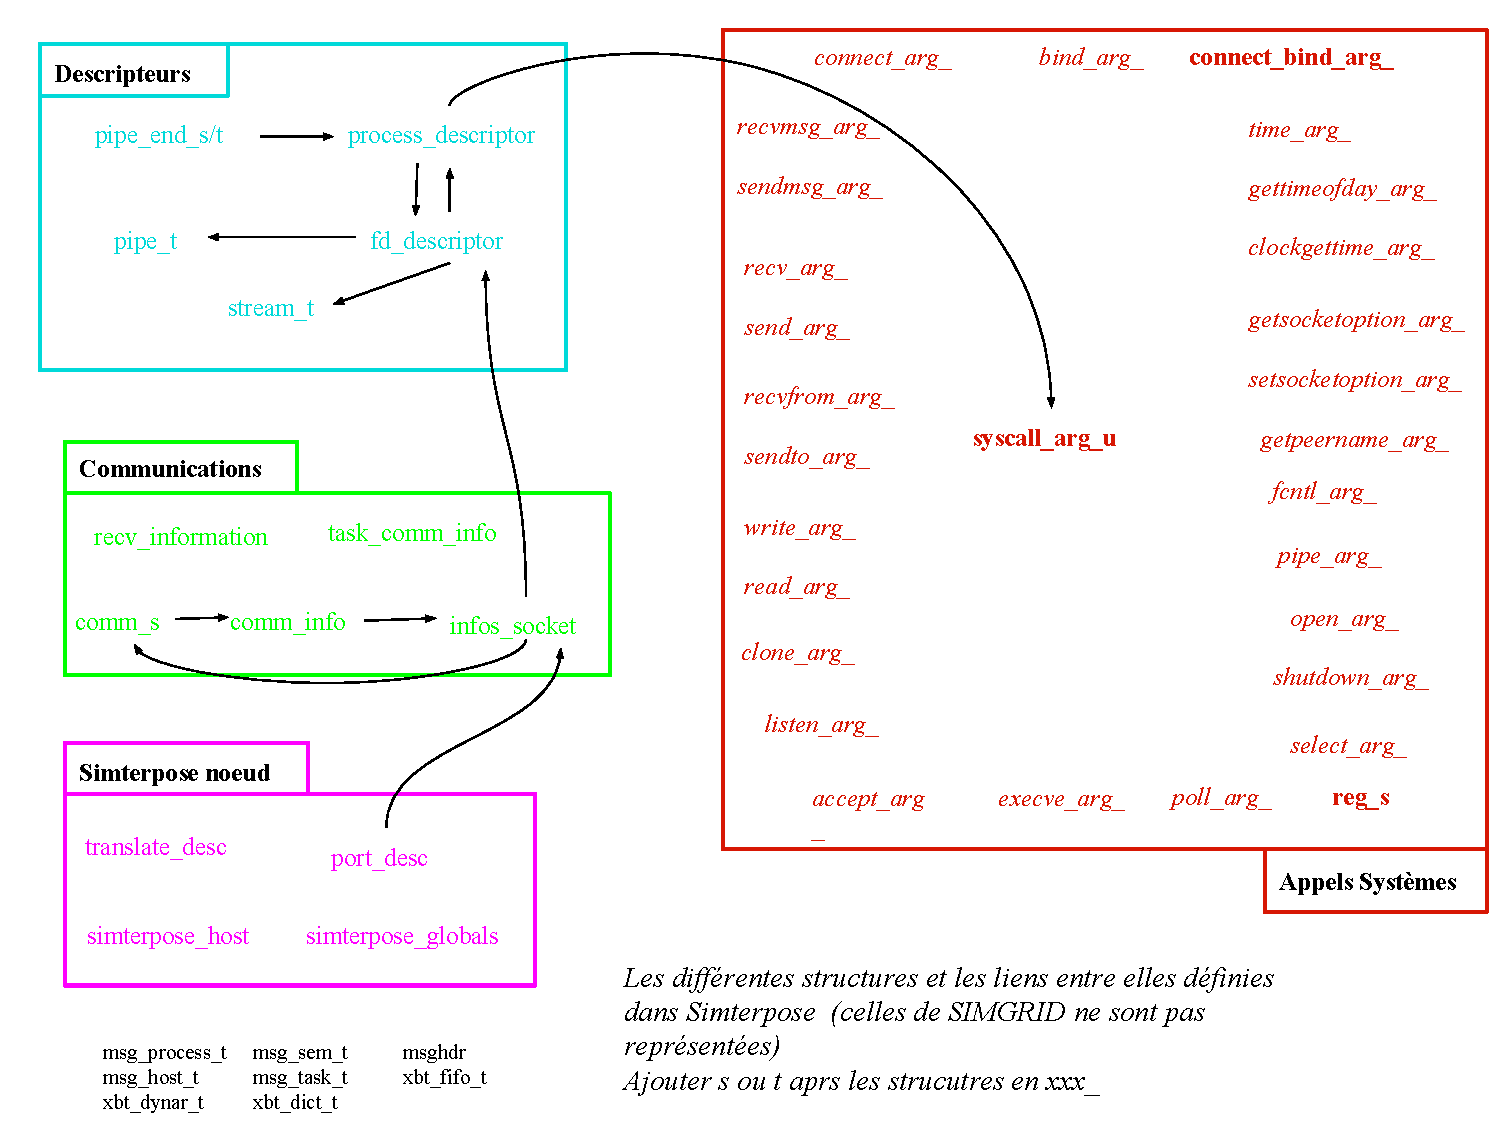
\includegraphics[scale=0.8]{Pictures/Linked_structures_Simteprose_V3.pdf}}
\end{landscape}

\end{document}
